\title{Das kleine Segel 1x1}
%\author{
%}
\date{\today}

\documentclass[12pt]{article}
\usepackage[utf8]{inputenc}

\usepackage{stmaryrd}
\usepackage{graphicx}

\begin{document}
\maketitle

\begin{abstract}
Dieser Text soll eine kurze Einführung in das Thema Segeln sein. Es ist dafür gedacht um im Segeln unerfahren die Grundbegriffe näher zu bringen, im mit einen erfahrenen Skipper eine längere Tour durchführen zu können.
\end{abstract}

\section{Begriffe}

\paragraph{Heck}
\paragraph{Bug}
\paragraph{Backbord}
\paragraph{Steuerbord}
\paragraph{Fallen}

\paragraph{Schoten}

\paragraph{Wanden und Stagen}

\section{Segel}

\begin{figure}[h!]
\begin{center}
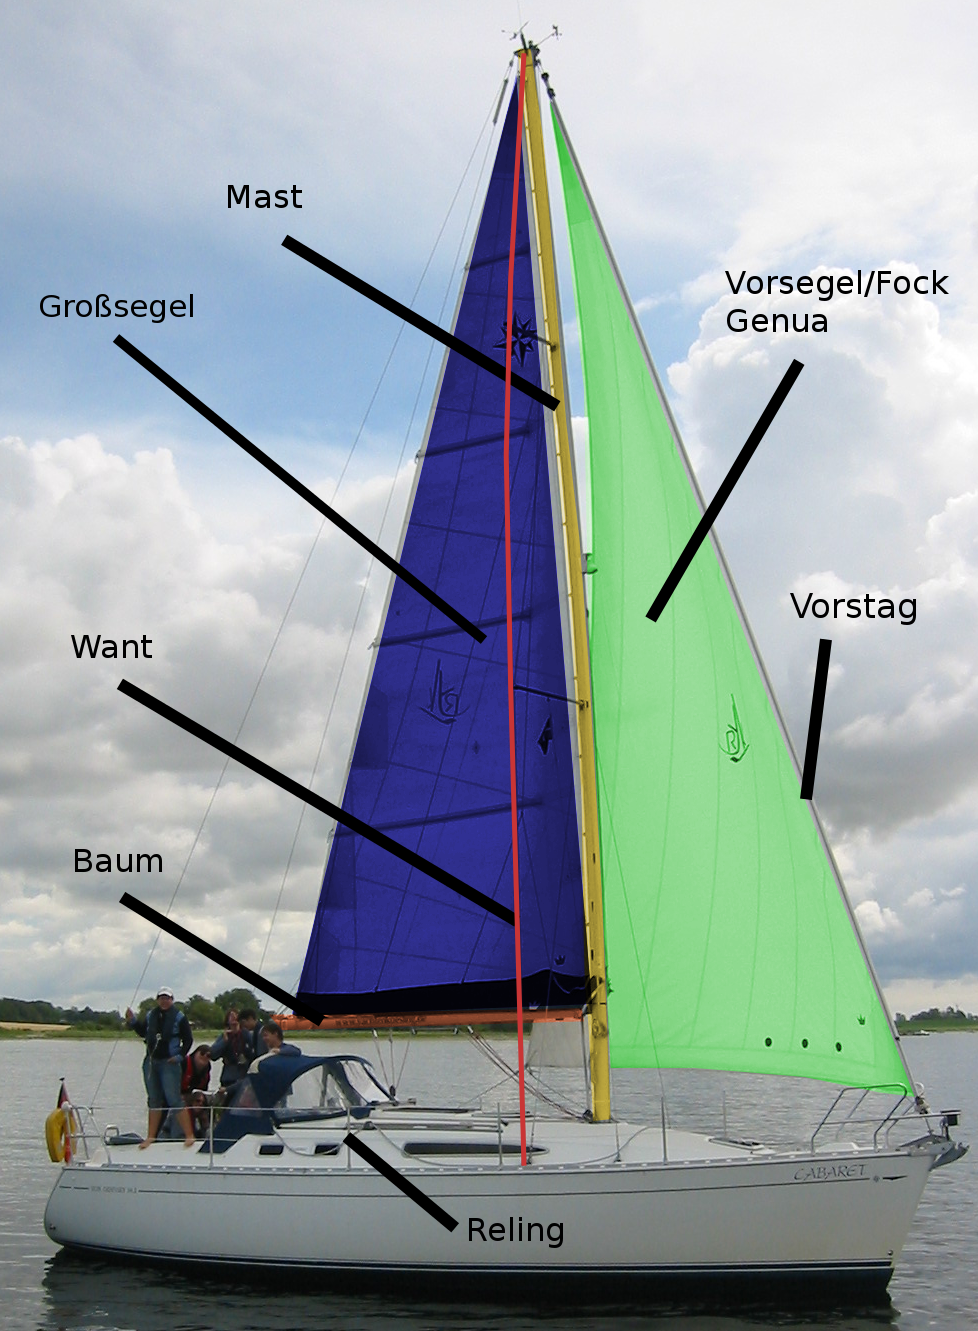
\includegraphics[scale=0.3]{bilder/yacht.png}
\end{center}
\caption{Die Segel einer Yacht}
\end{figure}

\section{Packliste}
Dies ist eine Liste der Sachen an die man unbedingt denken muss. Sie ist nur als Referenz zu nutzen und erhebt keinen Anspruch auf Vollständigkeit.

\begin{itemize}
\renewcommand{\labelitemi}{$\boxempty$}
\item Gummistiefel
\end{itemize}

\end{document}
